\section{Durchführung}
\label{sec:Durchführung}

\begin{figure}[H]
    \centering
    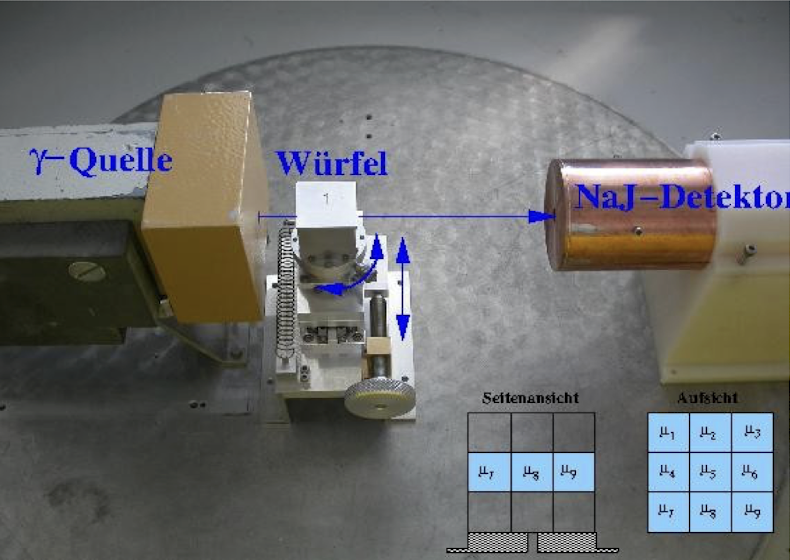
\includegraphics[scale=0.35]{Abbildungen/Aufbau.pdf}
    \caption{Schematischer Aufbau des Versuchs.\cite{V46}}
    \label{fig:aufbau}
\end{figure}

Der Aufbau des Versuchs ist in \autoref{fig:aufbau} dargestellt.
Als Lichtquelle wird eine Halogen-Lampe verwendet, welche ein überwiegend infrarotes Emissionsspektrum liefert, da der verwendete Halbleiter
GaAs durchlässig für infrarotes Licht ist.
Die Strahlung fällt zunächst durch eine Linse um möglichst parallele Lichtstrahlen zu erzeugen.
Ein Lichtzerhacker in Form einer sich drehenden Sektorscheibe befindet sich als nächstes im Strahlengang um das Licht in Impulse zu zerlegen.
Danach trifft das Licht auf ein Glan-Thompson-Prisma, dessen Aufgabe es ist, das Licht linear zu polarisieren.
Die Funktionsweise eines Glan-Thompson-Prismas ist schematisch in \autoref{fig:prisma} dargestellt. Die Polarisationsebenen der beiden
austretenden Strahlen stehen orthogonal aufeinander.
\begin{figure}[H]
    \centering
    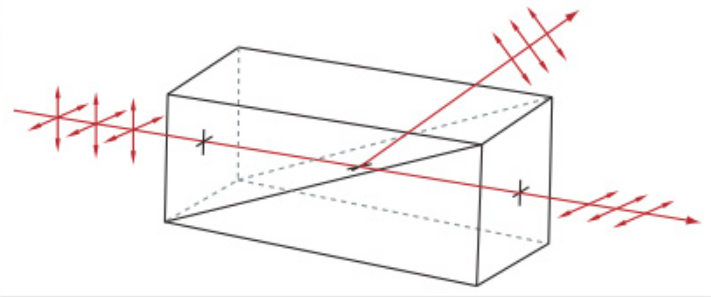
\includegraphics[scale=0.35]{Abbildungen/prisma.png}
    \caption{Strahlengang in einem Glan-Thompson-Prisma.\cite{Prisma}}
    \label{fig:prisma}
\end{figure}
Am Prisma befindet sich zudem ein Goniometer zur Winkelmessung.
Das Licht tritt dann durch den Spalt zwischen den Elektromagneten und durch die Probe, die sich in einem Luftspalt in den Elektromagneten
befindet.
Der Wellenvektor des Lichtfeldes ist hierbei parallel zum zeitlich konstanten Magnetfeldvektor, der durch die Elektromagneten erzeugt wird.
Die Elektromagneten sind an einen Polwender angeschlossen, der dafür sorgt, dass keine gefährlichen Induktionsspannungen beim Umpolen enststehen.
Nach den Elektromagneten passiert das Licht einen Interferenzfilter, wo eine bestimmte Wellenlänge des Lichts herausgefiltert wird.
Das Licht ist nun monochromatisch und wird in einem weiteren Glan-Thompson-Prisma in
zwei zueinander senkrecht polarisierte Komponenten zerlegt.
Mithilfe von Sammellinsen werden die beiden Strahlen nun auf Photowiederstände gelenkt, welche die Intensität messen.
Die entstehenden Signale gelangen nun an einen Differenzverstärker, dessen Ausgangsspannung proportional zur Differenz der beiden Eingangsspannungen
ist und somit verschwindet, wenn beide Eingangsspannungen in Betrag und Phase übereinstimmen.
Der darauf folgende Selektivverstärker wird auf die durch den Lichtzerhacker erzeugte
Modulationsfrequenz abgestimmt, sodass Störfrequenzen bestmöglich herausgefiltert werden.

\subsection{Justage des Versuchsaufbaus}
\label{sub:Justage}

\subsection{Messung zur Bestimmung der Drehwinkel}
\label{sub:Drehwinkel}

\subsection{Messung zur Bestimmung der Magnetfeldstärke}
\label{sub:Magnetfeld}




